\section{Introduzione}
\subsection{ASGAL}
ASGAL (Alternative Splicing Graph Aligner) \cite{ASGAL} è un tool per l'identificazione di eventi di Alternative Splicing espressi in un campione di RNA-seq a partire da un'annotazione di un gene. ASGAL si compone di tre step:

\begin{itemize}
	\item \textbf{Costruzione dello splicing graph}: a partire dall'annotazione di un gene, ASGAL costruisce uno splicing graph, ovvero una struttura a grafo che rappresenta tutti i trascritti noti del gene in input.
	\item \textbf{Allineamento Splice-Aware}: ASGAL allinea le read di RNA-Seq con lo splicing graph del gene in input. L'allineamento è Splice-Aware in quanto è necessario tenere traccia della posizione di esoni ed introni per un corretto allineamento.
	%\item \textbf{Computazione degli allineamenti Spliced}: gli allineamenti prodotti dallo step precedente vengono convertiti nel formato SAM
	\item \textbf{Rilevamento degli eventi di Alternative Splicing}: gli allineamenti prodotti dallo step precedente sono analizzati per rilevare gli eventi di alternative splicing indotti dalle read del campione.
\end{itemize}


\begin{figure}[h!]
	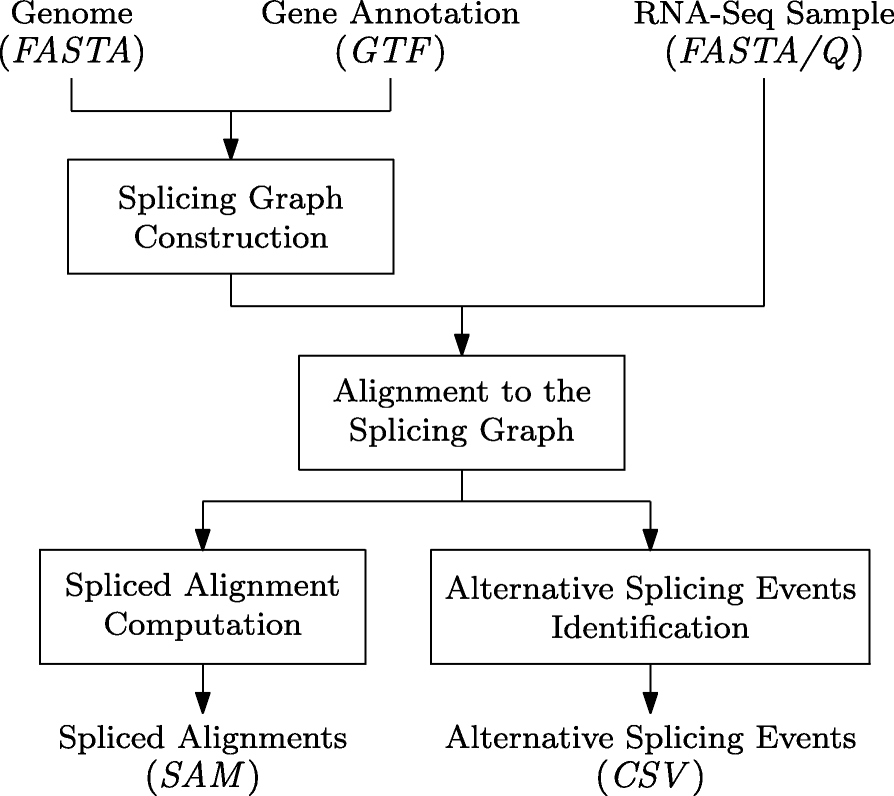
\includegraphics[height=12cm,width=\textwidth]{images/asgal.png}
  \caption{La pipeline di ASGAL illustrata}
  \label{fig:ASGAL}
\end{figure}
